\chapter{Supernova Neutrino Bursts and Low-energy Neutrinos}
\label{ch:physics-snblowe}

\section{Overview}
\label{sec:physics-snblowe-overview}

The DUNE experiment will be sensitive to neutrinos in the few to few
tens of MeV range, which create short tracks potentially accompanied
gamma ray and other secondary particle signatures.  This regime is of
particular interest for detection of the burst of neutrinos from a
core-collapse supernova (the primary focus of this section), and
neutrinos from other astrophysical sources are also potentially detectable.
The low-energy event regime has particular reconstruction, background and triggering challenges.

\subsection{Expected  Signal}

A core-collapse supernova\footnote{``Supernova'' always
  refers to a ``core-collapse supernova'' in this chapter unless
  stated otherwise.} occurs when a massive star reaches the end of its
life, and stellar burning can no longer support the star's weight.
This catastrophic collapse results in a compact remnant such as a
neutron star, or possibly a black hole, depending on the mass of the
progenitor.  The infall is followed by a ``bounce'' when sufficiently
high core density is reached, and in some unknown (but non-zero)
fraction of cases, the shock wave formed after the bounce results in a
bright explosion~\cite{Janka:2012wk}.  The explosion energy represents
only a small fraction of the enormous total gravitational binding
energy of the resulting compact remnant, however --- thanks to the
neutrinos' weak coupling, which allows them to escape --- within a few
tens of seconds almost all of the energy is emitted in the form of
neutrinos in the tens-of-MeV range.  In spite of their weak coupling,
the neutrinos are copious enough to (very likely) play a significant
role in the explosion.

Neutrinos from the celebrated SN1987A core
collapse~\cite{Bionta:1987qt,Hirata:1987hu} in the Large Magellanic
Cloud outside the Milky Way were observed; however, the
statistics %of this observation
were sparse %enough that
and a great many questions remain.  A high-statistics observation of a
nearby supernova neutrino burst would be possible with the current
generation of detectors. Such an observation would shed light
on %very many questions about
the nature of the astrophysical event, as well as on the nature of
neutrinos themselves.  Sensitivity to the different flavor components
of the flux is highly desirable.

The core-collapse neutrino signal starts with a short, sharp
\emph{neutronization} (or \emph{break-out}) burst primarily composed of
$\nu_e$ (originating from $p+e^- \rightarrow n + \nu_e$, as protons
and electrons get squeezed together), and is followed by an
``accretion'' phase lasting some hundreds of milliseconds, as matter falls onto the collapsed core.  The later
``cooling'' phase over $\sim$10~seconds represents the main part of
the signal, over which the proto-neutron star sheds its gravitational
binding energy.  The neutrino flavor content and spectra change
throughout these phases, and the supernova's temperature evolution can
be followed with the neutrino signal.
% (see
%Figure~\ref{fig:temp_comparison}). 
Some fairly generic supernova
signal features are illustrated in Figure~\ref{fig:spectrum}, based on~\cite{Fischer:2009af} and reproduced from~\cite{Wurm:2011zn}.
% Last three cases can be quite complicated, especially last
%
\begin{figure}[!htb]
\centering
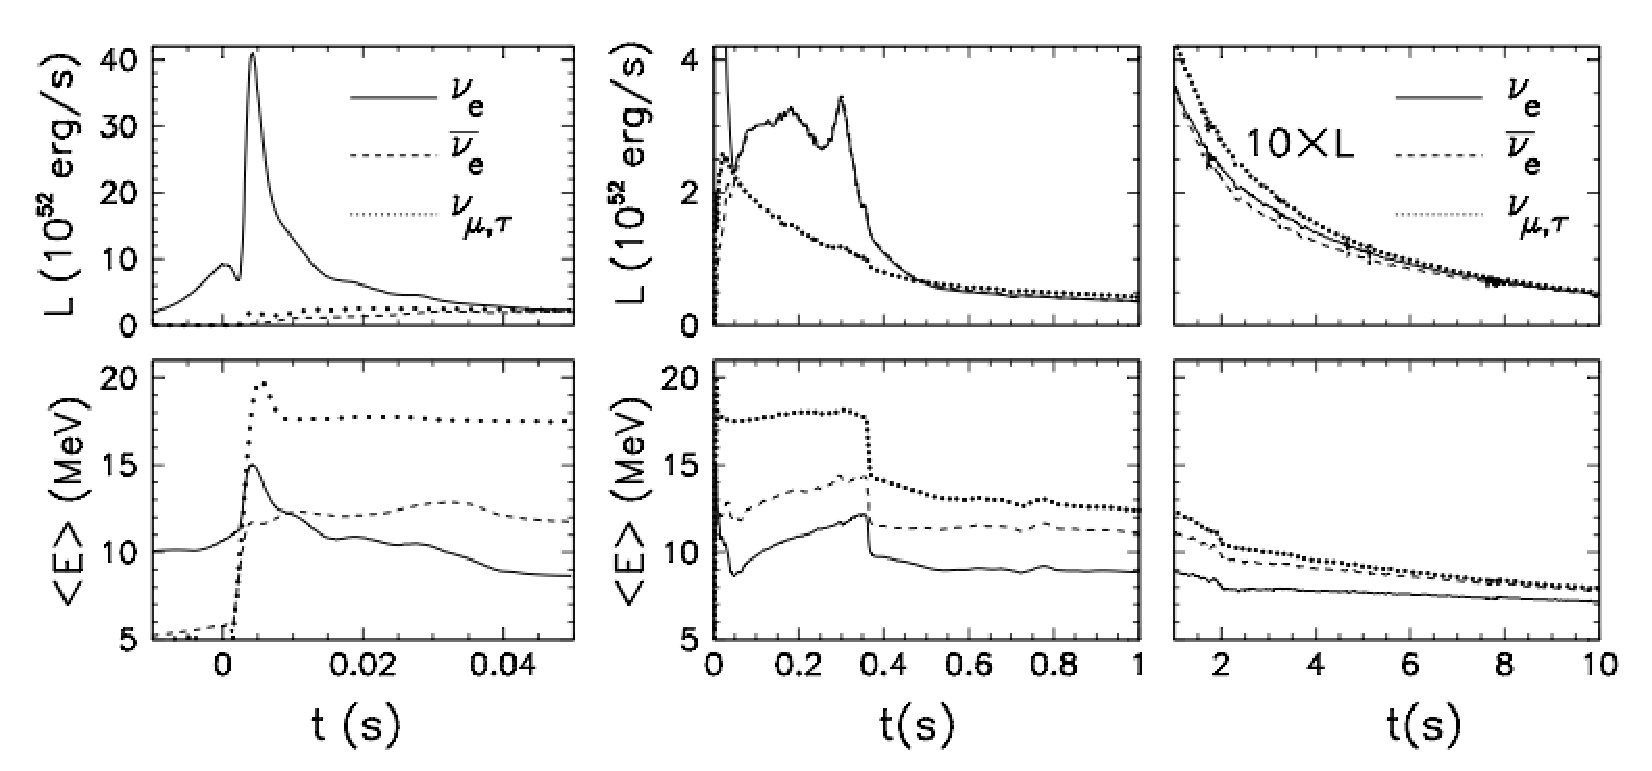
\includegraphics[width=0.9\textwidth]{basel_flux.pdf}
\caption[Expected core-collapse neutrino signal]{Expected
  core-collapse neutrino signal from the ``Basel''
  model~\cite{Fischer:2009af}, for a
  10.8 $M_{\cdot}$ progenitor.  The left plots show the very early
  signal, including ``neutronization burst;'' the middle plots show
  the ``accretion phase'', and the right plots show the cooling
  phase. Across the top, luminosities as a function of time are shown. 
  Across the bottom, the plots show average energy as a function of time for the
  $\nu_e$, $\overline{\nu}_e$ and $\nu_{\mu,\tau}$ flavor components of the
  flux (fluxes for $\nu_\mu$, $\overline{\nu}_\mu$, $\nu_\tau$,
  and $\overline{\nu}_\tau$ should be identical).  Figure courtesy of~\cite{Wurm:2011zn}.}
\label{fig:spectrum}
\end{figure}

The supernova neutrino spectrum at a given moment in time is expected
to be well described by a
parameterization~\cite{Minakata:2008nc,Tamborra:2012ac} given by:
\begin{equation}
        \label{eq:pinched}
        \phi(E_{\nu}) = \mathcal{N} 
        \left(\frac{E_{\nu}}{\langle E_{\nu} \rangle}\right)^{\alpha} \exp\left[-\left(\alpha + 1\right)\frac{E_{\nu}}{\langle E_{\nu} \rangle}\right] \ ,
\end{equation}
where $E_{\nu}$ is the neutrino energy, $\langle E_\nu \rangle$ is the
mean neutrino energy, $\alpha$ is a ``pinching parameter'', and
$\mathcal{N}$ is a normalization constant.
%
Large $\alpha$ corresponds to a more ``pinched'' spectrum (suppressed
high-energy tail). This parameterization is referred to as a
``pinched-thermal'' form. The different $\nu_e$, $\overline{\nu}_e$ and
$\nu_x, \, x = \mu, \tau$ flavors are expected to have different
average energy and $\alpha$ parameters and to evolve differently in
time. 


\subsection{Detection Channels and Interaction Rates}

Luquid argon should have a particular sensitivity to the $\nu_e$
component of a supernova neutrino burst, via charged-current
absorption of $\nu_e$ on $^{40}$Ar.  Cross sections for the most
relevant interactions are shown in Fig.~\ref{fig:xscns}.
% I have some improved figures somewhere...

\begin{figure}[!htb]
\centering
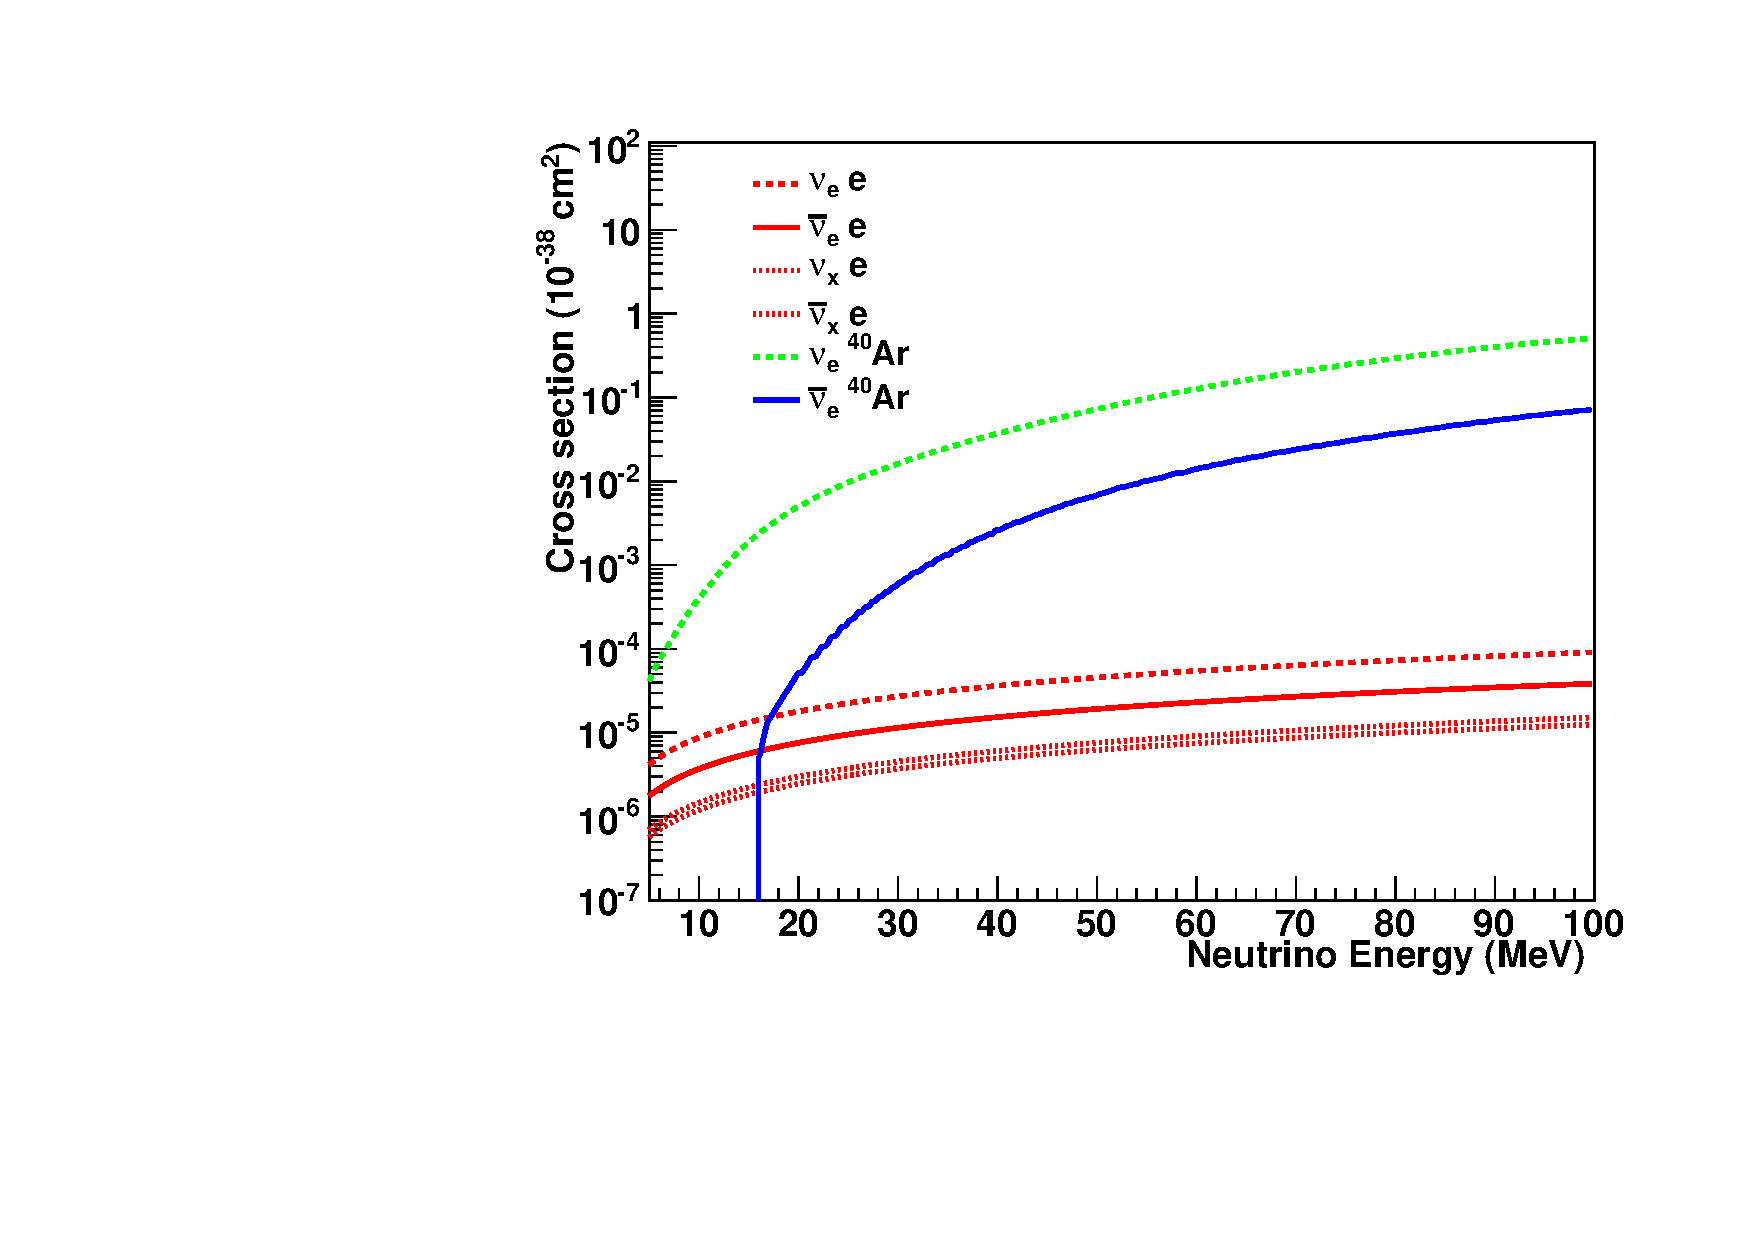
\includegraphics[width=0.6\textwidth]{argon_xscn.pdf}
\caption[]{Cross sections for supernova-relevant interactions in argon.}
\label{fig:xscns}
\end{figure}
%
The predicted event rate from a supernova burst may be calculated by
folding expected neutrino differential energy spectra in with cross
sections for the relevant channels, and with detector response.
%


Table~\ref{tab:argon_events} shows rates calculated  for the dominant interactions in argon for
the ``Livermore'' model~\cite{Totani:1997vj}, and the ``GKVM''
model~\cite{Gava:2009pj}.  Figure~\ref{fig:eventrates} shows the
expected observed differential event spectra for these fluxes.  Clearly, the $\nu_e$
flavor dominates.
%
\begin{table}[!htb]
  \caption[Event rates for different models in \SI{34}{\kt} of LAr for
    a core-collapse at 10~kpc]{Event rates for different
    supernova models in \SI{34}{\kt} of liquid argon for a core collapse at 10~kpc, for $\nu_e$ and $\bar{\nu}_e$ charged-current channels and elastic scattering (ES) on electrons.
    Event rates will simply scale by active detector mass and inverse square of supernova distance.}
\label{tab:argon_events}\centering
\begin{tabular}{$L^c^c}%$
\toprule
\rowtitlestyle
Channel & Events & Events \\
\rowtitlestyle
& ``Livermore'' model & ``GKVM'' model  \\ 
\toprowrule

$\nu_e + ^{40}{\rm Ar} \rightarrow e^- + ^{40}{\rm K^*}$ & 2308  & 2848 \\ \colhline

$\overline{\nu}_e + ^{40}{\rm Ar} \rightarrow e^+ + ^{40}{\rm Cl^*}$ & 194 & 134\\ \colhline

$\nu_x + e^- \rightarrow \nu_x + e^-$                           & 296 &  178\\

%$\nu_x + ^{40}{\rm Ar} \rightarrow \nu_x+ ^{40}{\rm Ar}^*$ & & \\ \hline
\toprule
\rowtitlestyle
Total &  2794& 3160 \\ 
\bottomrule
\end{tabular}
\end{table}
%
\begin{figure}[!htb]
\centering
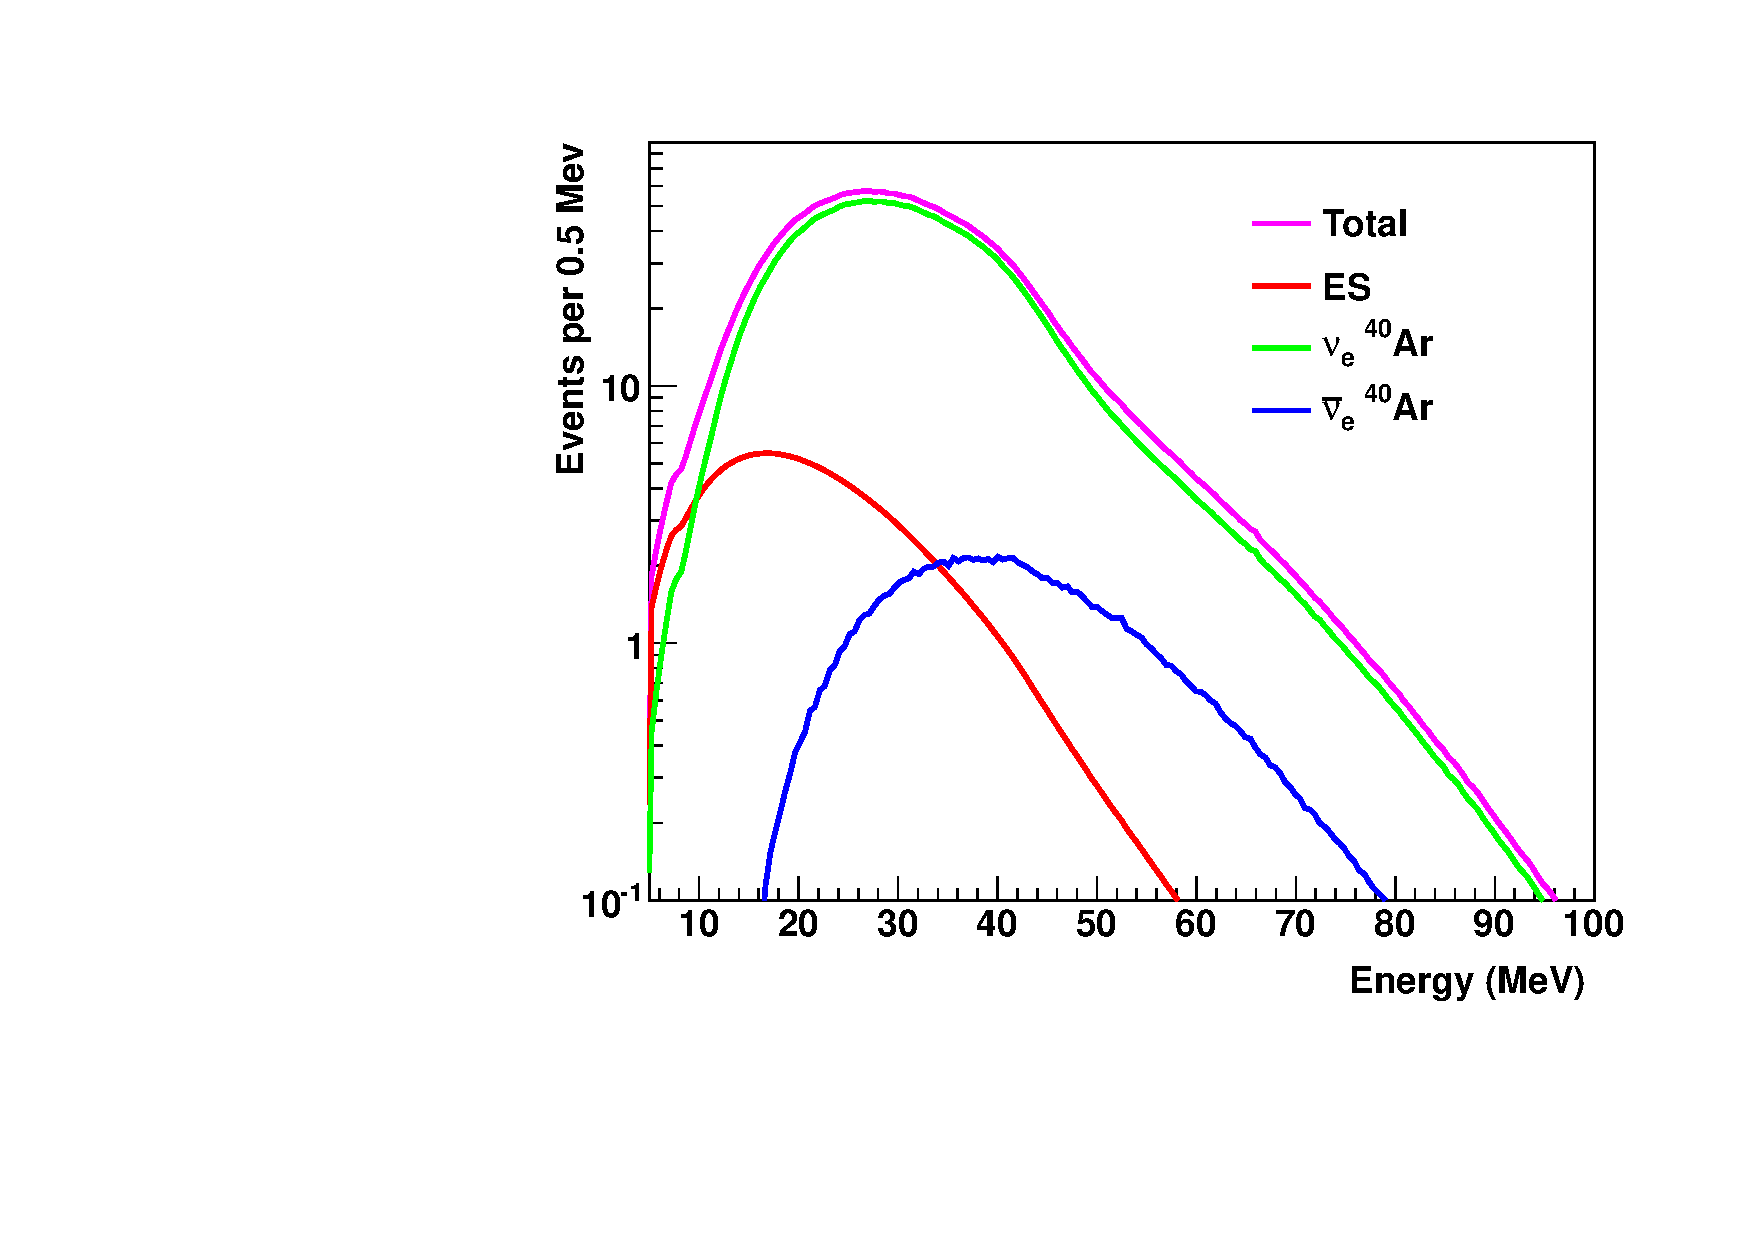
\includegraphics[width=2.0in]{interaction_rates_gvkm_ar34kt.pdf}
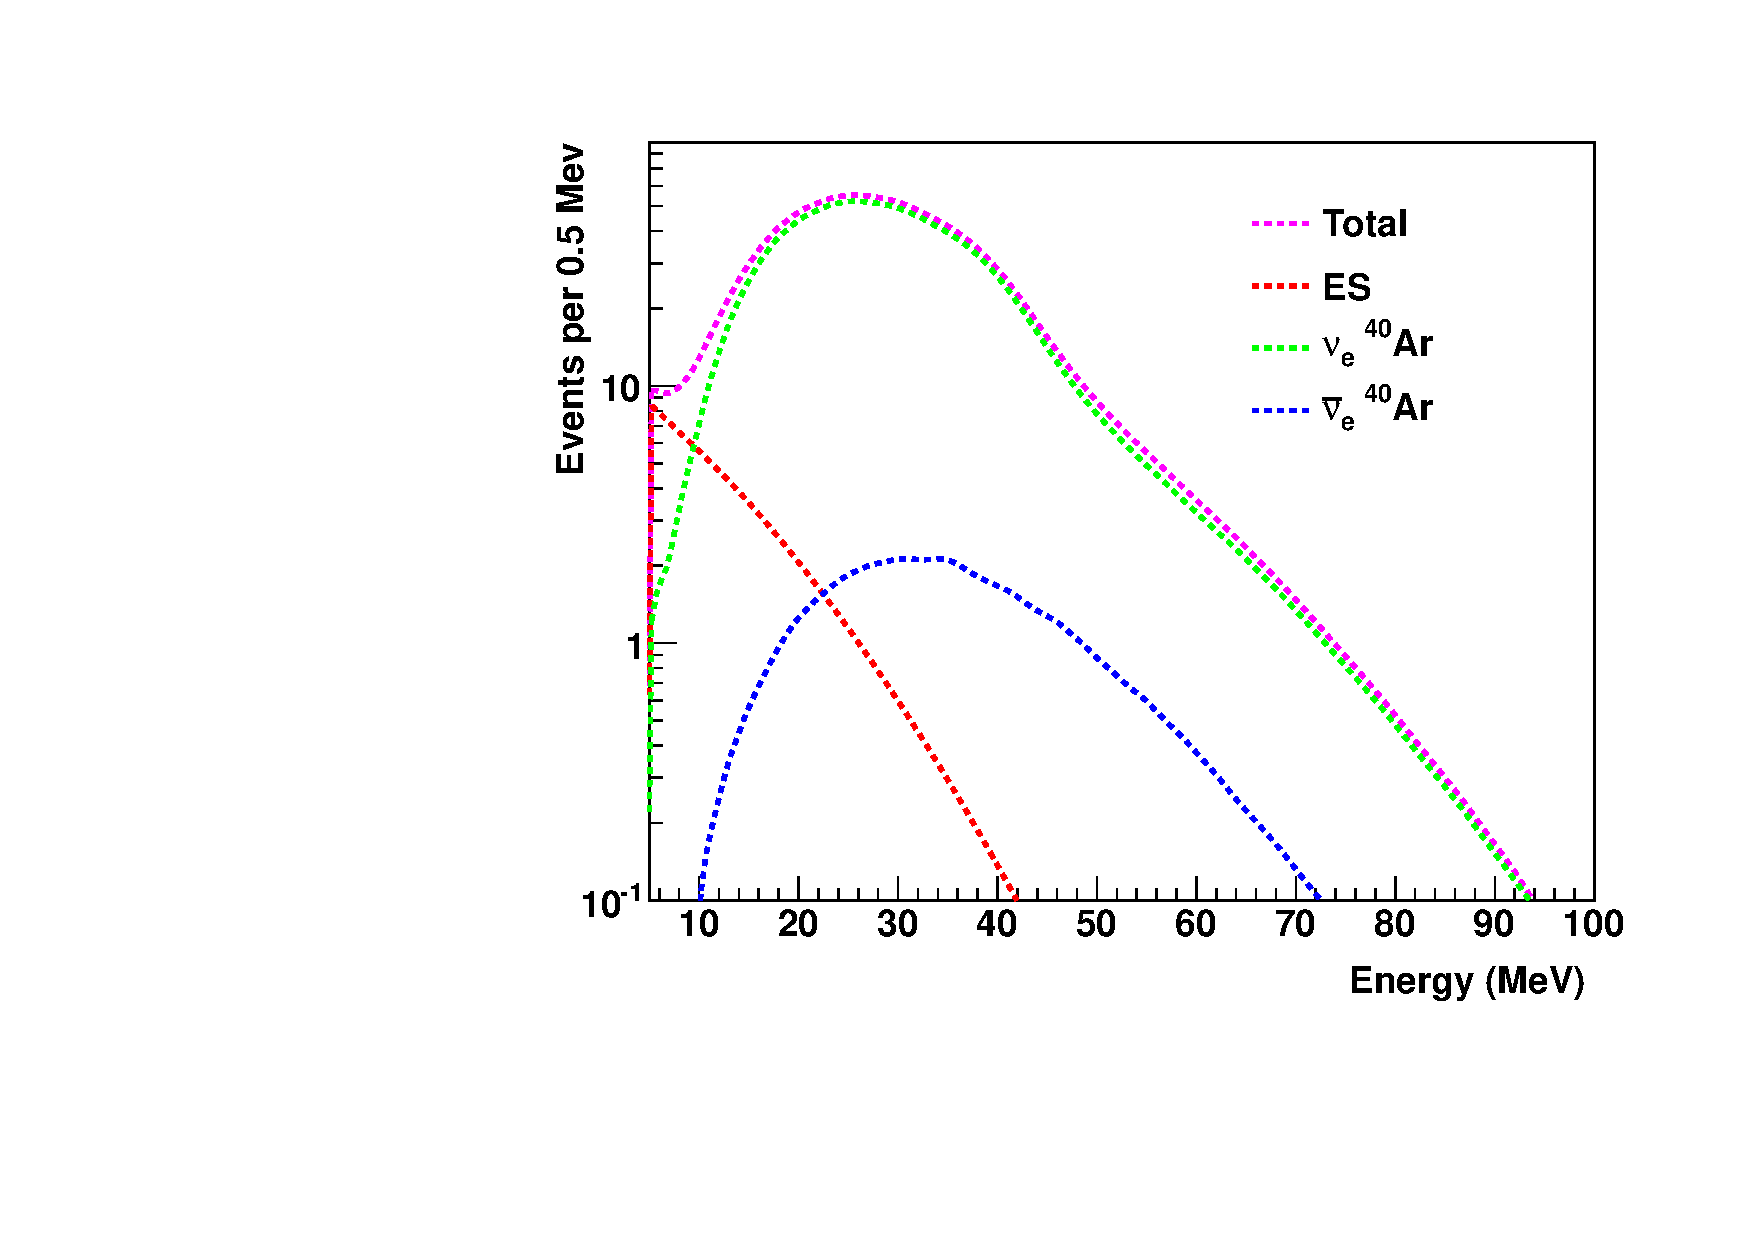
\includegraphics[width=2.0in]{smeared_rates_gvkm_ar34kt.pdf}
\vspace{-5pt}
\caption[SN $\nu$ event rates in \SI{34}{kt} of LAr for a core
  collapse at 10~kpc, GKVM]{Supernova neutrino event rates in 34~kt of argon for a core
  collapse at 10~kpc, for the GKVM model~\cite{Gava:2009pj} (events
  per 0.5~MeV), showing three relevant interaction channels. Left:
  interaction rates as function of true neutrino energy.  Right:
  ``smeared'' rates as a function of detected energy, assuming
  resolution from~\cite{Amoruso:2003sw}.}
  \label{fig:eventrates}
\end{figure}

Figure~\ref{fig:garching} gives another example of an expected burst
signal, for which a calculation with detailed time dependence of the
spectra is available~\cite{Huedepohl:2009wh} out to 9~seconds
post-bounce.  This model has relatively low luminosity but a robust
neutronization burst.  Note that the relative fraction of
neutronization-burst events is quite high.
%
\begin{figure}[!htb]
\centering
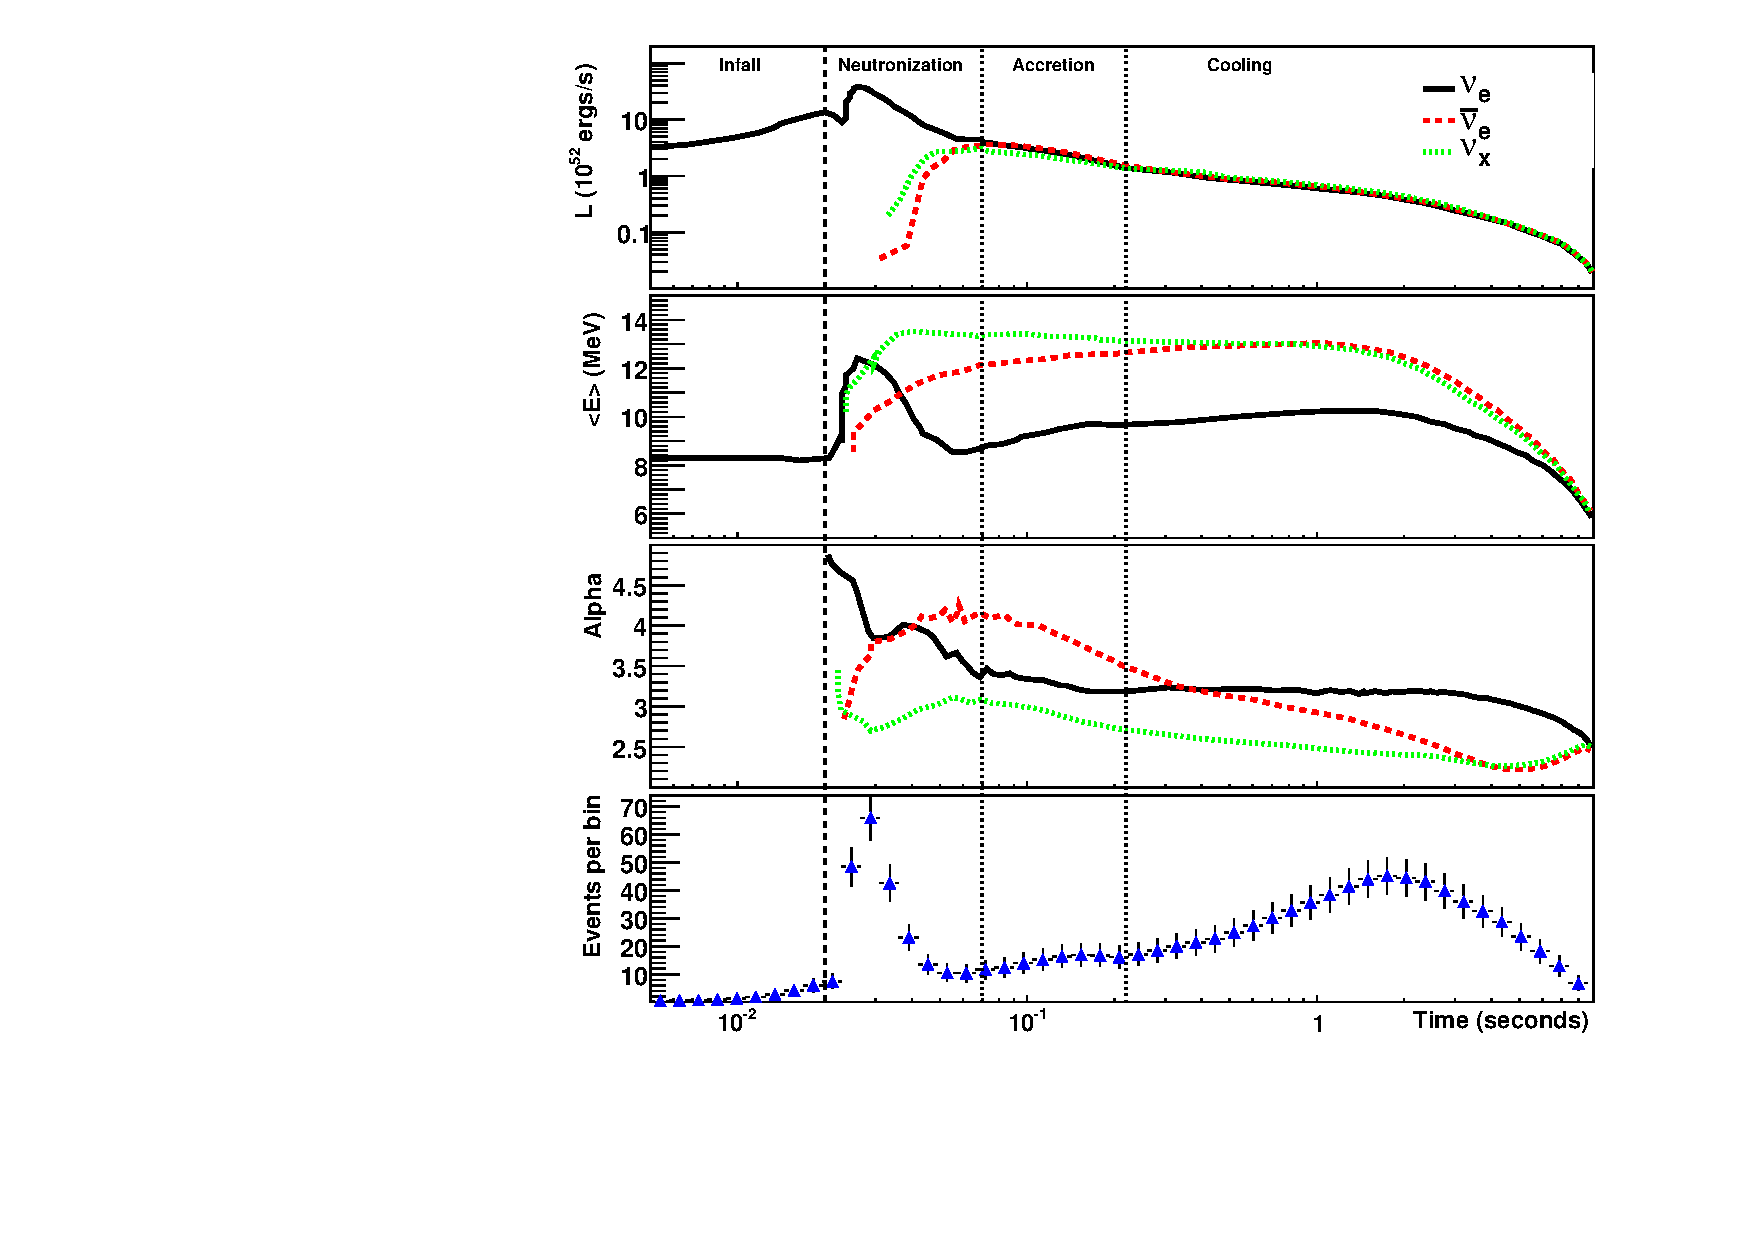
\includegraphics[width=0.9\textwidth]{garching.pdf}
\caption[Garching flux signal with neutronization burst]{ Expected
  time-dependent signal for a specific flux model for an
  electron-capture supernova~\cite{Huedepohl:2009wh} at 10~kpc.  The
  top plot shows the luminosity as a function of time, the second plot
  shows average neutrino energy, and the third plot shows the $\alpha$
  (pinching) parameter.  The fourth (bottom) plot shows the total number of
  events (mostly $\nu_e$) expected in 34 kt of liquid argon, calculated using
  SNoWGLoBES.  Note the logarithmic binning in time; the plot shows
  the number of events expected in the given bin and the error bars
  are statistical. The vertical dashed line at 0.02 seconds indicates
  the time of core bounce, and the vertical lines indicate different
  eras in the supernova evolution.  The leftmost time interval
  indicates the infall period.  The next interval, from core bounce to
  50~ms, is the neutronization burst era, in which the flux is
  composed primarily of $\nu_e$.  The next period, from 50 to 200~ms,
  is the accretion period. The final era, from 0.2 to 9~seconds, is
  the proto-neutron-star cooling period.  }
\label{fig:garching}
\end{figure}


\section{Neutrino Physics and Other Particle Physics}
\label{sec:physics-snblowe-neutrino-physics}


Neutrino oscillations modulate the flavor-energy-time evolution of the spectrum, including 
``collective'' effects due to neutrino-neutrino interactions.  A
voluminous literature exists exploring these collective phenomena,
e.g.,~\cite{Duan:2005cp,Fogli:2007bk,Raffelt:2007cb,Raffelt:2007xt,EstebanPretel:2008ni,Duan:2009cd,Dasgupta:2009mg,Duan:2010bg,Duan:2010bf}.

\textit{Update, more here}

Certain phenomena are even postulated to indicate
beyond-the-standard-model physics~\cite{Raffelt:1999tx} such as
axions, extra dimensions and an anomalous neutrino magnetic moment;
non-observation of these effects, conversely, would enable constraints
on these phenomena.


\textit{Add: absolute mass?}


\textit{From Alan: needs merging/trimming}
 In essence, neutrino oscillations offer observable signals for Lorentz and CPT violation because they compare the propagation of two flavors. Another class of tests in- volves comparing the propagation of neutrinos with other species or of neutrinos of the same flavor but different energies. These amount to time-of-flight or dispersion studies.
Time-of-flight and dispersion effects lack the interferometric resolving power available to neutrino oscillations, but they provide instead sensitivity to Lorentz- and CPT-violating effects that cannot be detected via oscillations. The corresponding SME coefficients controlling these ef- fects are called oscillation-free coefficients.
Supernova antineutrinos are of particular interest in this context because of the long baseline, which implies sensitivities many orders of magnitude better than available from time-of-flight measurements in beams. Ob- servations of the supernova SN1987A yield constraints on the difference between the speed of light and the speed of antineutrinos, which translates into constraints on isotropic and anisotropic coefficients in both the min- imal and nonminimal sectors of the SME. Knowledge of the spread of arrival times constrains the maxi- mum speed difference between SN1987A antineutrinos of different energies in the approximate range 10-40 MeV, which restricts the possible antineutrino dispersion and yields further constraints on SME coefficients.
Analyses of this type would be possible with DUNE if supernova neutrinos are observed. Key features to maximize sensitivity would include absolute timing information to compare with photon spectral observations and relative timing information for different components of the antineutrino energy spectrum. Significant improvements over existing limits are possible.
Figure 4 displays DUNE supernova sensitivities to coefficients for Lorentz and CPT violation that leave unaffected neutrino oscillations and so cannot be measured using atmospheric or long-baseline neutrinos. The figure assumes a supernova comparable to SN1987A but located elsewhere on the sky. Studies of supernova neutrinos using DUNE can measure many coefficients (green) at levels improving over existing limits (grey).

\begin{figure}[!htb]
\centering
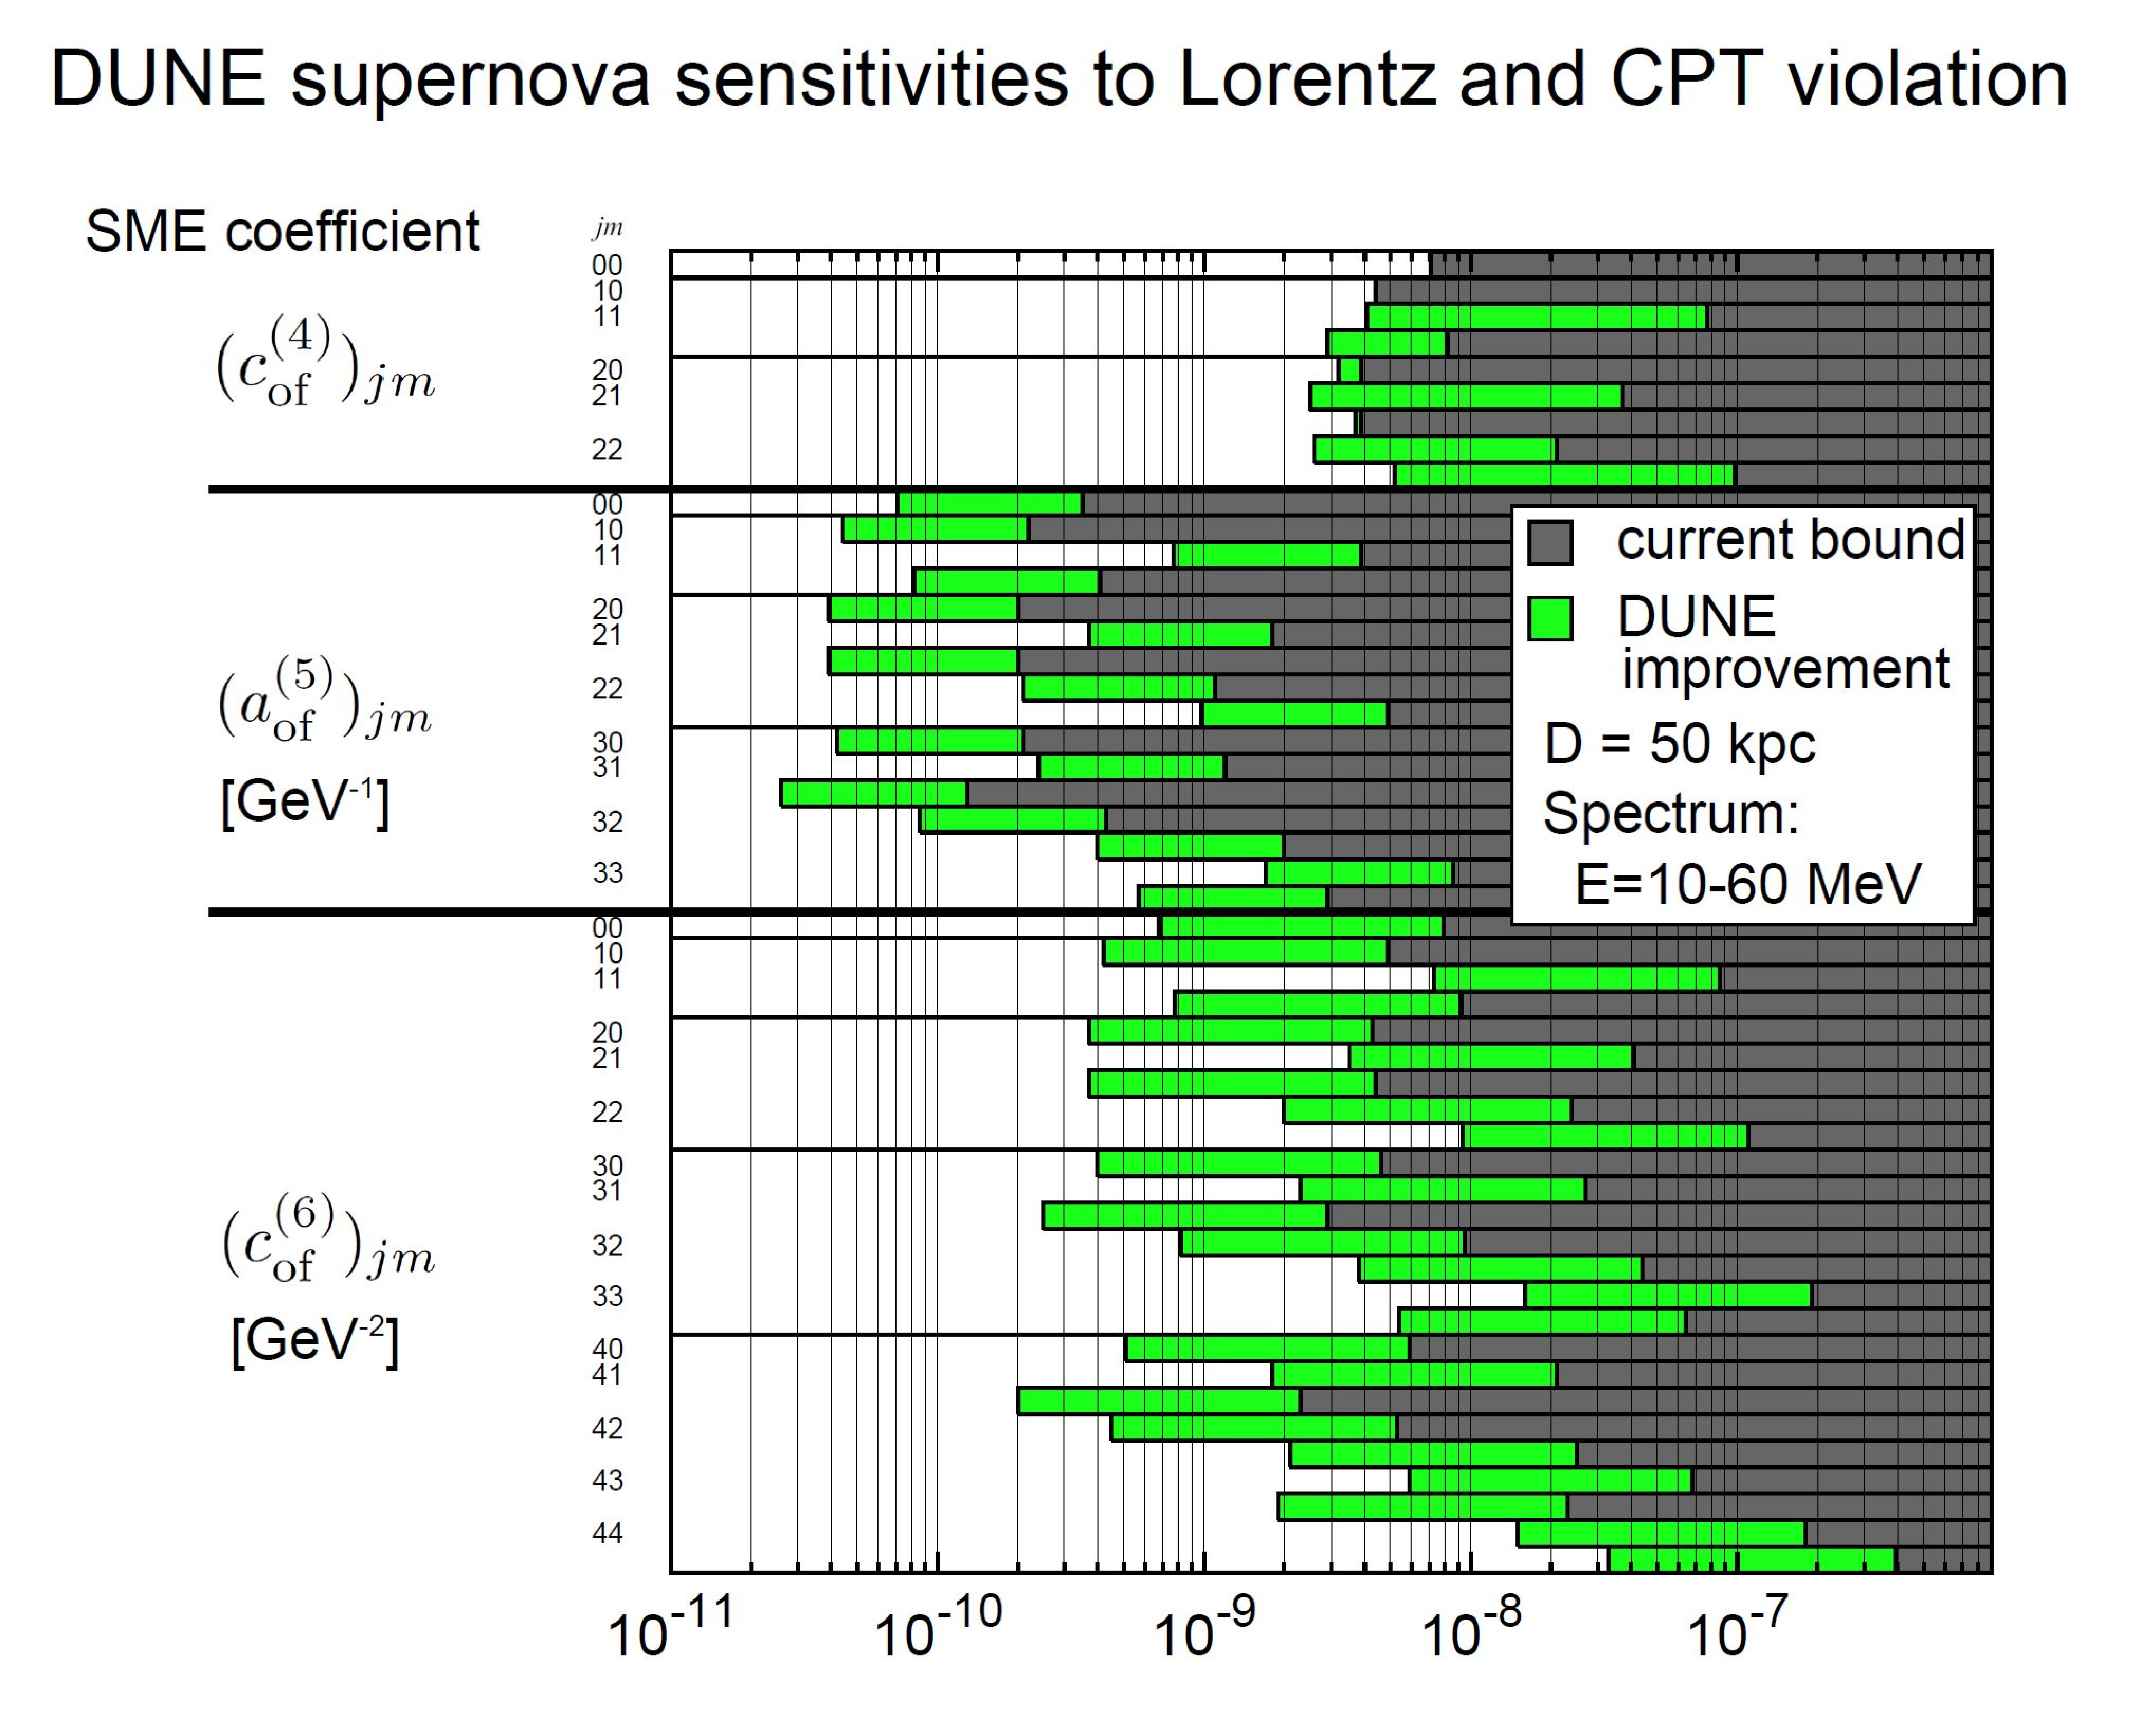
\includegraphics[width=0.9\textwidth]{DUNE-SME-SN.pdf}
\caption{DUNE supernova sensitivities to oscillation-free coefficients for Lorentz and CPT violation. Studies of DUNE supernova neutrinos can measure many coefficients (green) at levels improving over existing limits (grey). These Lorentz- and CPT- violating effects leave oscillations unchanged and so are unobservable in atmospheric or long-baseline measurements.}
\label{fig:snliv}
\end{figure}

\section{Astrophysics}
\label{sec:physics-snblowe-astrophysics}



A number of astrophysical phenomena associated with supernovae are expected to be observable
in the supernova neutrino signal, providing a remarkable window into the event, for example: 
\begin{itemize}
\item The initial burst, primarily composed of $\nu_e$ and called the
  ``neutronization'' or ``breakout''
  burst, %should be observable, although it
  represents only a small component of the total signal.  However,
  oscillation effects can manifest themselves in an observable manner
  in this burst, and flavor transformations can be modified by the
  ``halo'' of neutrinos generated in the supernova envelope by
  scattering~\cite{Cherry:2013mv}.
\item The formation of a black hole would cause a sharp signal cutoff
  (e.g.,~\cite{Beacom:2000qy,Fischer:2008rh}).
\item Shock wave effects (e.g.,~\cite{Schirato:2002tg}) would cause a
  time-dependent change in flavor and spectral composition as the
  shock wave propagates.
\item The standing accretion shock instability
  (SASI)~\cite{Hanke:2011jf,Hanke:2013ena}, a ``sloshing'' mode
  predicted by three-dimensional neutrino-hydrodynamics simulations of
  supernova cores, would give an oscillatory flavor-dependent
  modulation of the flux.
\item Turbulence effects~\cite{Friedland:2006ta,Lund:2013uta} would
  also cause flavor-dependent spectral modification as a function of
  time.
\end{itemize}

The supernova neutrino burst is prompt with respect to the
electromagnetic signal and therefore can be exploited to provide an
early warning to astronomers~\cite{Antonioli:2004zb,Scholberg:2008fa}.
Additionally, a liquid argon signal~\cite{Bueno:2003ei} is expected to
provide some pointing information, primarily from elastic scattering
on electrons.

Even non-observation of a burst, or non-observation of
a $\nu_e$ component of a burst in the presence of supernovae (or other
astrophysical events) observed in electromagnetic or gravitational
wave channels, would still provide valuable information about the
nature of the sources.  Further, a long-timescale, sensitive search
yielding no bursts will also provide limits on the rate of
core-collapse supernovae.


% r-process

\section{Detector Requirements}
\label{sec:physics-snblowe-detector-requirements}

This may need more than the 1 page allocated.

Energy Resolution

Time Resolution

Angular Resolution

Particle ID, tagging

Backgrounds

Triggering, DAQ, Data Rate


\section{Additional Astrophysical Neutrinos}
\label{sec:physics-snblowe-other}

\subsection{Solar Neutrinos}

Intriguing questions in solar neutrino physics remain,
even after data
from the Super-K and SNO~\cite{Fukuda:2001nj,Ahmad:2001an}
experiments explained the long-standing mystery of missing solar
neutrinos~\cite{Cleveland:1998nv} as due to flavor
transformations. 
Some unknowns, such as the fraction of energy production via the CNO
cycle in the Sun, flux variation due to helio-seismological modes that
reach the solar core, or long-term stability of the solar core
temperature, are astrophysical in nature. Others directly impact
particle physics. Can the MSW model explain the amount of flavor
transformation as a function of energy, or are non-standard neutrino
interactions required?  Do solar neutrinos and reactor antineutrinos
oscillate with the same parameters? 
% Experimental data expected in the
%immediate future (e.g., further data from
%Borexino~\cite{Borexino7be:2011} and Super-K as well as 
%SNO+~\cite{Kraus:2006qp}) will address some questions, but the
%high-statistics measurements necessary to further constrain
%alternatives to the standard oscillation scenario may need to wait fo

Detection of solar and other low-energy neutrinos is challenging in
a LArTPC because of high intrinsic detection energy thresholds for
the charged-current interaction on argon ($>$\SI{5}{\MeV}). To be
competitive, this physics requires either a very low visible energy
threshold ($\sim$\SI{1}{\MeV}) or a very large mass (\SI{50}{\kt}).
However, compared with other technologies, a LArTPC offers a large
cross section and unique signatures from de-excitation
photons. Aggressive R\&D efforts in low-energy triggering and
control of background from radioactive elements may make detection
in DUNE possible, and a large detector mass would make the pursuit
of these measurements worthwhile.

Signatures of solar neutrinos in DUNE
are elastic scattering on electrons as well as CC absorption of $\nu_e$ on $^{40}$Ar, which has a 4.5-MeV energy threshold.
In Table~\ref{tab:solarnu} the solar neutrino event rate in a
\ktadj{34} LArTPC is shown, assuming a \MeVadj{4.5} neutrino energy
threshold and 31\% $\nu_e$.
%
\begin{table}[!htb]
\caption[Solar neutrino rates in a LArTPC]{Solar neutrino event rates in a \ktadj{34} LArTPC assuming 
a \MeVadj{4.5} neutrino energy threshold and 31\% $\nu_e$}
\label{tab:solarnu}
\begin{tabular}{$L^c}%$
\toprule
\rowtitlestyle
Transition & Rate (evts/day) \\ \toprowrule
Fermi  & 31 \\ \colhline
Gamow-Teller & 88 \\ \bottomrule
\end{tabular}
\end{table}


The solar neutrino physics potential of a large LArTPC depends
primarily on its energy threshold, which will 
be determined by the ability to pick up a low-energy electron, light collection of the photon-triggering system,
and background suppression. 
In any
detector of this kind, the decay of the naturally occurring $^{39}$Ar
produces $\beta$'s with a \keVadj{567} endpoint and an expected rate
of \SI{10}{\MHz} per \SI{10}{\kt} of liquid argon. This limits the
fundamental reach of DUNE to neutrino interactions with visible
energies above \SI{1}{\MeV}. 
Cosmic-muon and fast-neutrino
interactions with the $^{40}$Ar nucleus (which are rather complex
compared to interactions on $^{16}$O or $^{12}$C) are likely to
generate many long-lived spallation products that could limit the
detection threshold for low-energy neutrinos.
Studies of the spallation background in the DUNE LArTPC are
underway. 

% The production rate of $^{40}$Cl, a beta emitter with an
% endpoint of \SI{7.48}{\MeV} that is a dominant source of background at
% energies above \SI{5}{\MeV}, is shown in Figure~\ref{fig:cl40bkgd} as
% a function of depth.
% %
% \begin{figure}[!htb]
% \centering\includegraphics[width=0.7\textwidth]{figures/cosmicbkgd_40clrate.pdf}
% \caption[$^{40}$Cl production rates produced by (n,p) reaction per depth, \SI{10}{\kt}]{$^{40}$Cl production rates in a \ktadj{10} detector produced by (n,p) reaction as a function of depth.}
% \label{fig:cl40bkgd}
% \end{figure}
% %
% The cosmogenic background rates as a function of
% beta kinetic energy from several other beta emitters at the \SIadj{4850}{\ft} 
% level of Sanford Underground Research Facility are shown in Figure~\ref{fig:cosmicbkg}.
% %
% \begin{figure}[!htb]
% \centering
% \includegraphics[width=0.7\textwidth]{smyfig/solarmsw.pdf}
% \caption[Measurements of the solar MSW transition]{Measurements of the solar MSW transition. The red band combines
% SK and SNO $^8$B data~\cite{Aharmim:2011vm}, the green measurements
% of $^7$Be and pep are from Borexino~\cite{Borexino7be:2011,Borexinopep:2011} and the
% red error bar is Borexino's $^8$B measurement~\cite{Borexino8b:2008}. The 
% blue $pp$ point and the yellow error bar (CNO) combine all solar data. MSW resonance
% curves for three different parameters are overlaid.}
% \label{fig:solmsw}
% \end{figure}


The ICARUS collaboration has reported a \MeVadj{10}
threshold~\cite{Guglielmi:2012}. Assuming the %DUNE far 
detector itself
has low enough radioactivity levels, this threshold level would enable
a large enough detector to measure the electron flavor component of
the solar $^8$B neutrino flux with high statistical accuracy. It could % and
thereby further test the MSW flavor transformation curve with higher statistical precision and
potentially better energy resolution. 
In addition to these solar
matter effects, solar 
neutrinos also probe terrestrial matter effects
with the variation of the $\nu_e$ flavor observed with solar zenith
angle while the Sun is below the horizon --- the day/night effect (reported recently in ~\cite{Renshaw:2013dzu}). 

% A
% sizable effect is predicted only for the highest solar-neutrino
% energies, so while the comparatively high energy threshold is a
% handicap for testing the solar MSW resonance curve, it has a smaller
% impact on the high-statistics test of terrestrial matter
% effects. Recently, indication of the existence of the terrestrial
% matter effects were reported~\cite{Renshaw:2013}. Measurements of this
% effect currently give the best constraints on the solar mass ($\Delta
% m_{21}^2$) splitting 
% %(see Figure~\ref{fig:daynight}) 
% using neutrinos
% rather than antineutrinos~\cite{Gando:2013}.
%
% \begin{figure}[!htb]
% \centering\includegraphics[width=0.8\textwidth]{figures/sk_dn_vs_dm21.png}
% \caption[Solar neutrino day/night effect and dependence on $\Delta
% m^2_{21}$]{Dependence of the measured day/night asymmetry (fitted
%   day/night amplitude times the expected day/night asymmetry in red) on
%   $\Delta m^2_{21}$, for $\sin^2 \theta_{12}=0.314$ and $\sin^2
%   \theta_{13}=0.025$.  The 1$\sigma$ statistical uncertainties from
%   the recent measurements by \superk{} are given by the light
%   grey band. The additional dark grey width to the band shows the
%   inclusion of the systematic uncertainties. Overlaid are the 1$\sigma$ 
% allowed ranges from the solar global fit (solid green) and
%   the KamLAND experiment (dashed blue). Figure is courtesy of~\cite{Renshaw:2013}}
% \label{fig:daynight}
% \end{figure}

The comparison
of neutrino disappearance to antineutrino disappearance tests CPT
invariance. For good sensitivity to either solar-neutrino measurement,
a liquid argon far detector of at least \SI{34}{\kt} is required.


\subsection{Diffuse Supernova Background Neutrinos}

Galactic supernovae are relatively rare, occurring somewhere between
once and four times a century. In the Universe
at large, however, thousands of neutrino-producing explosions occur
every hour.  The resulting neutrinos --- in fact most of the neutrinos
%which have ever been 
emitted by all the supernovae since the onset of stellar formation ---
suffuse the Universe.  Known both as \emph{supernova relic neutrinos
  (SRN)} and as the \emph{diffuse supernova neutrino background
  (DSNB)}, their energies are in the few-to-\MeVadj{30} range.  SRN
have not yet been observed, but an observation would greatly enhance
our understanding of supernova-neutrino emission and the overall
core-collapse rate.


A liquid argon detector such as DUNE''s far detector is sensitive to
the $\nu_e$ component of the diffuse relic supernova neutrino flux,
whereas water Cherenkov and scintillator detectors are sensitive to
the antineutrino component.  However, backgrounds in liquid argon are as
yet unknown, and a huge exposure ($>$\SI{500}{\ktyr}s)
would likely be required for observation.  Given a detector of the
scale required to achieve these exposures (\SIrange{50}{100}{\kt})
together with tight control of
backgrounds, %with the appropriate technology,
DUNE --- in the long term --- could %eventually (Anne removed; redundant )
lay a unique and
  complementary role in the physics of relic neutrinos.

%
In the current DUNE design, the irreducible background from solar
neutrinos will limit the search for these relic neutrinos to an energy
threshold greater than \SI{18}{MeV}.  Similarly, a search for relic
antineutrinos is limited by the reactor antineutrino background to a
threshold greater than $\sim$\SI{10}{MeV}. The lower threshold and the
smaller average $\nu_e$ energy relative to that for antineutrinos
%\ (see
%Figure~\ref{fig:pred_srnspec}) 
leads to the need for a larger detector
mass.

A small but dedicated industry devotes itself to trying to predict the
flux of these relic supernova neutrinos here on
Earth~\cite{Totani:1995dw,Sato:1997sc,Hartmann:1997qe,Malaney:1996ar,Kaplinghat:1999xi,Ando:2005ka,Lunardini:2006pd,Fukugita:2002qw}. 
% Examples
% of two different predicted SRN spectra are shown in
% Figure~\ref{fig:pred_srnspec}, along with some of the key physics
% backgrounds from other neutrino sources.
% %
% \begin{figure}[!htb]
%      \centering\includegraphics[width=.8\textwidth]{smyfig/relicplot.pdf}
%      \caption[Relic supernova spectra and key neutrino
%      backgrounds]{Predicted relic supernova $\nu_e$ spectra from two
%        different models (red and blue) and some key neutrino
%        backgrounds: $^8$B solar $\nu_e$ (green), hep solar $\nu_e$
%        (cyan) and atmospheric $\nu_e$ (magenta).}
%      \label{fig:pred_srnspec}
% \end{figure}

In the DUNE LArTPC, relic supernova electron neutrinos would be
detected primarily via the charged current process as described by
Equation~\ref{eqn:srninteract}. The electron track should be
accompanied by evidence of ionization from the de-excitation of the
potassium, e.g., shorter tracks sharing a common vertex; this is
expected to help reduce backgrounds, but a detailed study has not yet
been undertaken.  In water Cherenkov and scintillator detectors, it is
the electron-antineutrino SRN flux that is detected through the
process of inverse-beta decay.  Unlike inverse-beta decay, for which
the cross section is known to the several-percent level in the energy
range of interest~\cite{Vogel:1999zy,Strumia:2003zx}, the cross
section for neutrino interactions on argon is uncertain at the 20\%
level~\cite{Ormand:1994js,Kolbe:2003ys,SajjadAthar:2004yf}. Another
limitation is that the solar {\em hep} neutrinos which have an                
endpoint at \SI{18.8}{\MeV}, will determine the lower bound of the SRN
search window ($\sim$ \SI{16}{\MeV}).  The upper bound is determined
by the atmospheric ${\nu}_{e}$ flux 
%as shown in
%Figure~\ref{fig:pred_srnspec} and 
is around \SI{40}{MeV}.
%While the LArTPC provides a unique sensitivity
%to the electron-neutrino component of the SRN flux, early studies
%indicate that the lower bound on the neutrino energy imposed by solar
%neutrinos implies that a huge mass of LAr --- \SI{100}{\kt} --- is
%required to get more than 4$\sigma$ evidence for the diffuse supernova
%flux in five years~\cite{Cocco:2004ac}. 
Although the LArTPC provides a unique sensitivity to the
electron-neutrino component of the SRN flux, early studies indicate
that due to this lower bound of $\sim$ \SI{16}{\MeV} DUNE would need a huge
mass of liquid argon --- of order \SI{100}{\kt} --- to get more than 4$\sigma$
evidence for the diffuse supernova flux in five
years~\cite{Cocco:2004ac}.
%
The expected number of relic
supernova neutrinos, $N_{\rm SRN}$, that could be observed in a
\SIadj{100}{\kt} LArTPC detector in five years~\cite{Cocco:2004ac}
assuming normal hierarchy is:
\begin{equation}
N_{\rm SRN} = 57 \pm 12  \ \ \ 16 \, {\rm MeV} \leq E_e \leq 40 \, {\rm MeV}
\label{eqn:srnrate}
\end{equation}
where $E_e$ is the energy of the electron from the CC interaction as
shown in Equation~\ref{eqn:srninteract}. The estimate of the SRN rate
shown in Equation~\ref{eqn:srnrate} has a weak dependence on the value
of $\sin ^2 \theta_{13}$. The above calculation is valid for values of
$\sin ^2 \theta_{13} > 10^{-3}$.  The main challenge for detection of such
a low rate of relic neutrinos in a LArTPC is understanding how much of
the large spallation background from cosmic-ray interactions with the
heavy argon nucleus (some of which are shown in Figure~\ref{fig:cosmicbkg}) leaks into the SRN search window. 
%the rate is higher given that $\sin^2 \theta_{13}$ is an order of
%magnitude larger than originally estimated.

\subsection{Other Low-Energy Neutrino Sources}

We note some other potential sources of signals in the tens-of-MeV range which may be observable in DUNE.  These include:
\begin{itemize}
\item Neutrinos from accretion disks~\cite{Caballero:2011dw}, black-hole/neutron star mergers~\cite{Caballero:2009ww}.  These will create spectra not unlike those from core-collapse events, and with potentially large fluxes but are even rarer.
\item ``Boosted'' dark matter

\end{itemize}

